\section{Microservice-Architekturen und Sicherheit}

Ein Microservice-basiertes System ist ein verteiltes System, das in der Regel auf mehreren Maschinen läuft. Auf jeder dieser Maschine laufen ein oder mehrere Microservices. Viele Teile des Systems müssen kommunizieren, entweder es werden Nachrichten bzw. Tasks entgegen genommen oder Nachrichten verschickt \cite{newman2015}. Ein breiter Angriffsvektor entsteht.

Dieses Kapitel beschreibt zunächst gängige Technologien zum Bau von Microservices. Anschließend werden Möglichkeiten betrachtet, koplexe Systeme auf Microservice-Basis zu ermöglichen. Die dabei entstehenden Herausforderungen werden hervorgehoben. Mögliche Ansätze zum Schutz eines Microservice-basierten Systems werden diskutiert.


\subsection{Technologien zum Bau von Microservices}

Ein Microservice sollte replizierbar (und somit skalierbar), sowie einfach zu deployen und sicher sein \cite{newman2015,microservicesIO}. Um Skalierbarkeit und einfaches Deployment zu erreichen, bietet es sich wiederum an Microservices in ähnlichen Ausführungsumgebungen laufen zu lassen. Das jedoch steht im Wiederspruch zu dem Konzept der Service-Unabhängigkeit und Autonomie. 

\subsubsection{Virtuelle Maschinen}
Mit herkömmlichen Virtualisierungstechnologien, wie etwa VMWare lässt sich die gewünschte Abstraktion schaffen. Services werden als Images für die virtuelle Maschine spezifiziert und können somit repliziert und portiert werden. Auch das Deployment des Services ist dann einfacher, weil nur noch das Service Image in der entsprechenden virtuellen Maschine (\textit{VM}) gestartet werden muss.

Wenn mehrere Microservices den gleichen Host oder die gleiche VM teilen, sind sie nicht unabhängig \cite{microservicesIO}. Bei böswilliger Manipulation oder Infiltrierung eines Services könnten auch andere Services im gleichen System beeinflusst werden. Folgt man dem Konzept so wäre es korrekt und sicher(-er) einen Service pro Host oder VM zu deployen. Das resultiert allerdings in Resourcen-Overhead der benötigt wird, um die (möglicherweise vielen) virtuellen Maschinen bzw. Hosts zu betreiben \cite{newman2015}. Die Grafik \ref{fig:container-vm} zeigt die Resourcen auf, die bei einem Setup mit virtuellen Maschinen benötigt werden und zeigt vergleichsweise den Resourcen-Verbrauch eines Container-basierten Setups.

\begin{figure}[h]
    \centering
    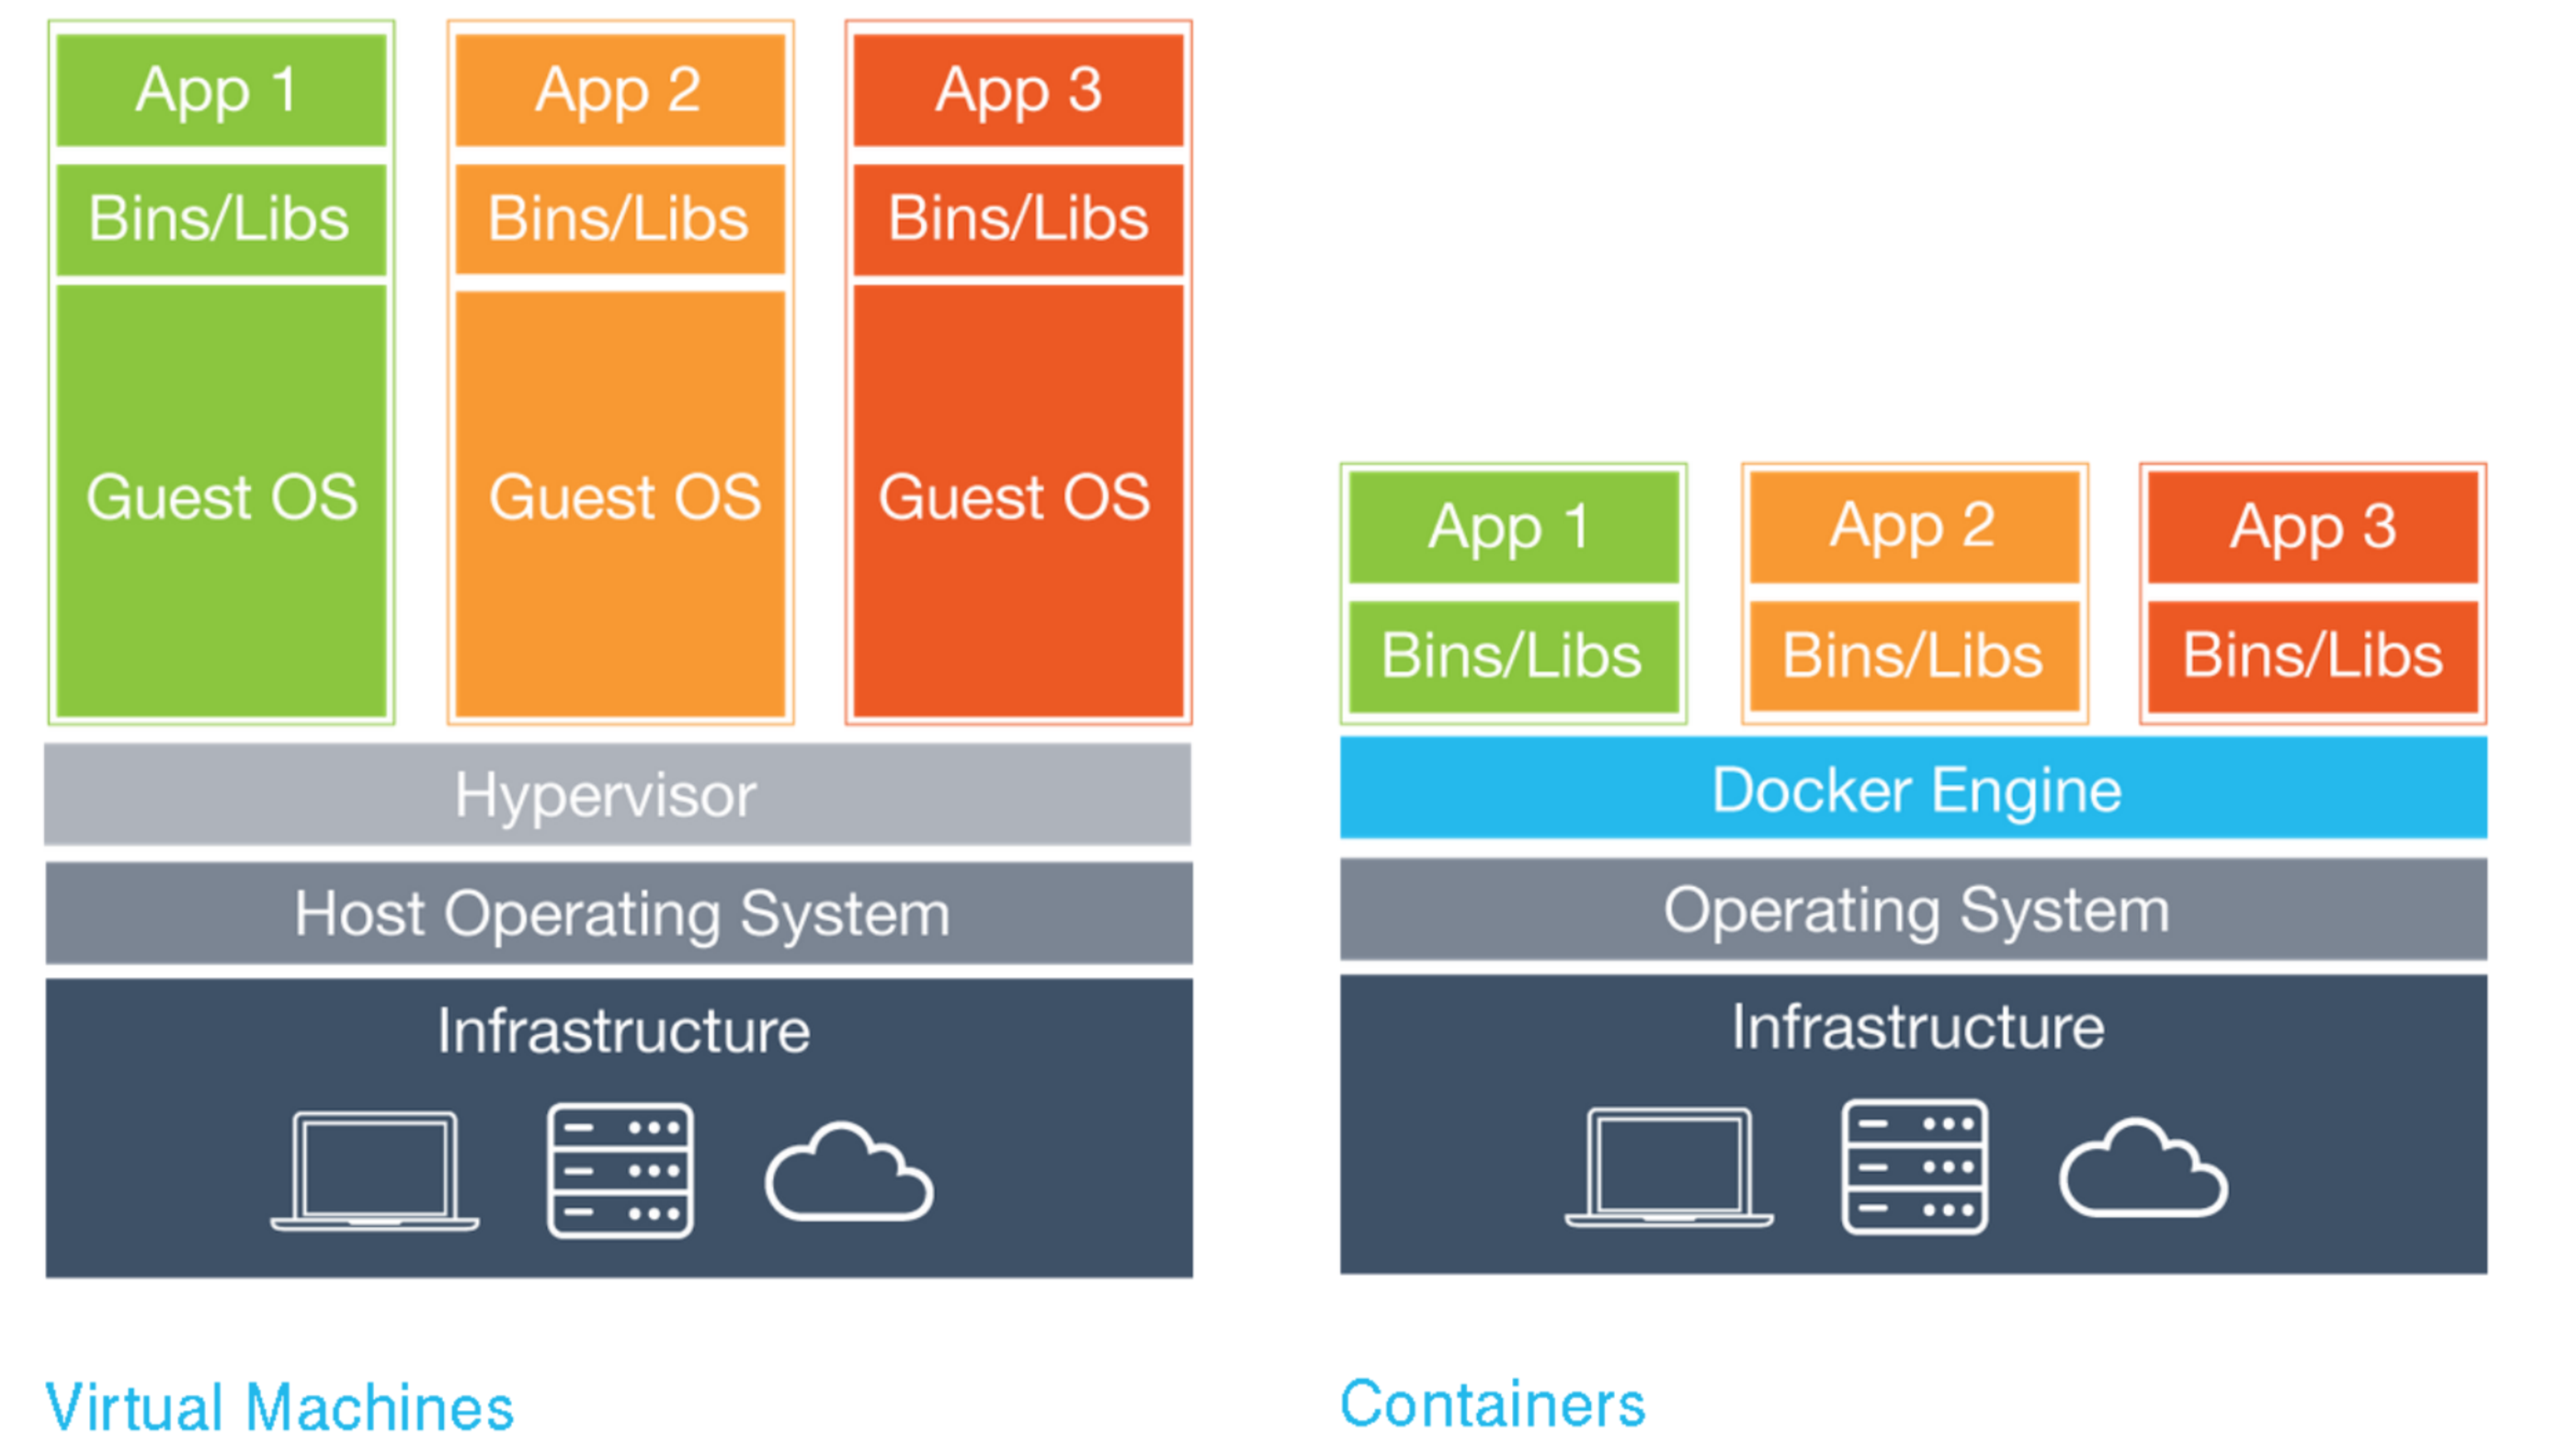
\includegraphics[scale=0.3]{img/container-vm.pdf}
    \caption{Vergleich von standard Virtualisierung und Docker Conainern, entnommen von \url{http://www.docker.com/what-docker}}
    \label{fig:container-vm}
\end{figure}

\subsubsection{Container}
Ein Container ist ein schlanker \glqq Wrapper\grqq\ um einen Linux Prozess. Wir betrachten hier Docker (\url{https://www.docker.com}) als Container Engine, es sei aber noch LXC (Linux Containers) erwähnt.

Docker und Docker-Container bieten ähnliche Funktionen wie eine virtuelle Maschine und zugehörige VM Images. Allerdings sind Container um ein Vielfaches leichtgewichtiger als VMs. Während eine VM ein Gast-Betriebssystem und eigene Libs enthält, enthalten Container nur eine Anwendung und deren benötigte Abhängigkeiten. Container teilen sich den Kernel des ausführenden Host-Betriebssystems und laufen als einzelner Prozess im Userland \cite{newman2015}. Die Grafik \ref{fig:container-vm} zeigt deutlich, auf welche Weise Container leichtgewichtiger sind als virtuelle Maschinen. Durch 

Zusätzlich werden Container durch Container Images spezifiert -- genauso wie bei VMs -- was die Verfielfältigung ungeheuer einfach macht. Allerdings ist die Modifikation von Dockerimages einfacher als das Ändern eines VM Images. Docker ermöglicht mithilfe eines sogenannten \textit{Dockerfile}s sehr einfache Manipulation von Images.

Allein die Charakteristika von Docker-Containern legen nahe, wie gut diese Technologie geeignet ist um die Anforderungen abzudecken, die eine Microservice-Architektur mit sich bringt. Durch das Design von Docker sind in Containern laufende Prozesse vollständig unabhängig voneinander. Services lassen sich in Form von Images einfach replizieren und portieren. Das ausführende System ist unwichtig, solange es ein Linux System ist und Docker installiert ist. Zum Thema Microservices, die mit Hilfe von Docker realisiert werden finden sich viele aktuelle Softwareprojekte.


\subsection{Managing Microservices / \glqq Orchestration\grqq}

Es gibt verschiedene Möglichkeiten, Microservices mit einander interagieren zu lassen um daraus ein komplexeres System entstehen zu lassen. Generell gilt für Microservices, dass sie \textit{klein}, auf \textit{eine Aufgabe} spezialisiert und \textit{autonom} sind \cite{newman2015}. Das bedeutet insbesondere auch, dass Services eines Systems einander meist nicht kennen. Das gängigste Problem in Microservice Architekturen ist die \textit{Service Discovery}. Um miteinander zu kommunizieren, müssen die Services sich zunächst in irgendeiner Form bekannt werden. Außerdem müssen Healthchecks vorhanden sein, um das Ausfallen einzelner Services beobachten zu können. Microservice Systeme, die produktiv genutzt werden sollen müssen auch Aufgaben wie Skalierung, Loadbalancing und natürlich Sicherheit im Sinne von \textit{Security} übernehmen. 

Es gibt viel Bewegung im Feld um Microservices und Docker. Viele großangelegte (Opensource-)Projekte, getrieben durch führende Software-Konzerne\footnote{\url{http://kubernetes.io}, \url{http://mesos.apache.org}, \url{http://azure.microsoft.com}, \url{https://aws.amazon.com/de/ecs/}} nehmen maßgeblich Einfluss auf die Softwareentwicklung in diesem Gebiet. 

Im Folgenden geben wir einen Kurzüberblick über Google Kubernetes. 